\documentclass[a4paper, 12pt]{article}
\usepackage[top=2cm, bottom=2cm, left=2.5cm, right=2.5cm]{geometry}
\usepackage[utf8]{inputenc}
\usepackage[brazilian]{babel}
\usepackage{indentfirst}
\usepackage{graphicx}
\usepackage{wrapfig}
\usepackage[pdftex]{hyperref}
\graphicspath{ {imagens/} }
\usepackage{xcolor}
% Definindo novas cores
\definecolor{verde}{rgb}{0.25,0.5,0.35}
\definecolor{jpurple}{rgb}{0.5,0,0.35}



\begin{document}
\begin{titlepage} %iniciando a "capa"
	\begin{center} %centralizar o texto abaixo
		{\large Unicamp}\\[0.2cm] %0,2cm é a distância entre o texto dessa linha e o texto da próxima
		{\large EM360}\\[0.2cm] % o comando \\ "manda" o texto ir para próxima linha
		{\large Prof. Antonio Bannwart}\\[3.2cm]
		{\bf \huge TERMODINÂMICA I}\\[5.1cm] % o comando \bf deixa o texto entre chaves em negrito. O comando \huge deixa o texto enorme
	\end{center} %término do comando centralizar
	{\large Erik Yuji Goto}\\[0.5cm] % o comando \large deixa o texto grande
	{\large RA: 234009}\\[10cm]
	\begin{center}
		{\large Campinas}\\[0.2cm]
		{\large 2020}
	\end{center}
\end{titlepage} %término da "capa"

\tableofcontents
\newpage

\section{Passo a Passo para Resolulção de Problemas}
	\begin{enumerate}
		\item Sistema Fechado ou Volume de Controle ?	
			\begin{itemize}
				\item Se sistema fechado, o processo ocorre de forma discreta (Q, W), em taxa ($ \dot{Q}, \dot{W} $) ou em ciclo?
				\item Se VC, opera em regime permanente ou transiente?
			\end{itemize}
		\item Esboçar o sistema fechado ou VC e indicar suas interações (trabalho, calor, massa)
		na fronteira com a vizinhança; indicar as propriedades conhecidas.
		\item Representar os estados percorridos pelo fluido em um diagrama de estado.
		\item Aplicar e simplificar as equações de balanço (massa, energia, entropia).
		\item Transformar as equações de balanço de forma a envolverem propriedades e
		interações conhecidas e procuradas
			\begin{itemize}
				\item Se a substância muda ou pode mudar de fase, buscar as propriedades dos estados fornecidos
				nas tabelas dessa substância (interpolar, se necessário).
				\item Se for gás ideal, usar as equações do modelo de gás ideal e decidir entre modelo com calores
				específicos constantes ou uso da tabela A-22 (ar como gás ideal).
				\item Se for substância incompressível, usar as equações desse modelo e o valor do calor específico.
			\end{itemize}
		\item Resolver as equações nas incógnitas do problema.
	\end{enumerate}

\newpage
\section{Capítulo 1 - Conceitos Introdutórios e Definições}

\subsection{A Linguagem da Termodinâmica}
	\begin{enumerate}
		\item \textbf{Sistema Fechado:} É uma quantidade fixa de substância (sempre a mesma) escolhida para análise. Não há troca de massa.
			\begin{figure}[h]
				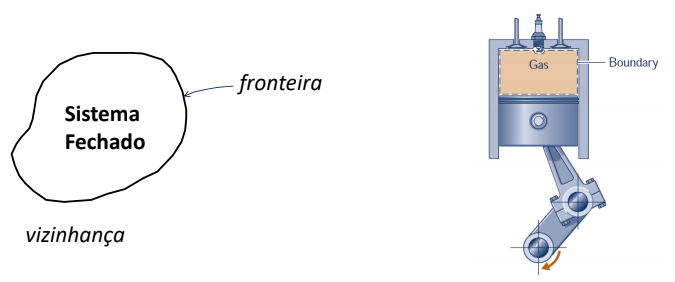
\includegraphics[width=10cm]{sf.png}
				\centering
				\caption{Sistema Fechado}
			\end{figure}
		
		\item \textbf{Volume de Controle:} É uma região do espaço por onde um ou mais fluidos \textbf{escoam}.
			\begin{figure}[h]
				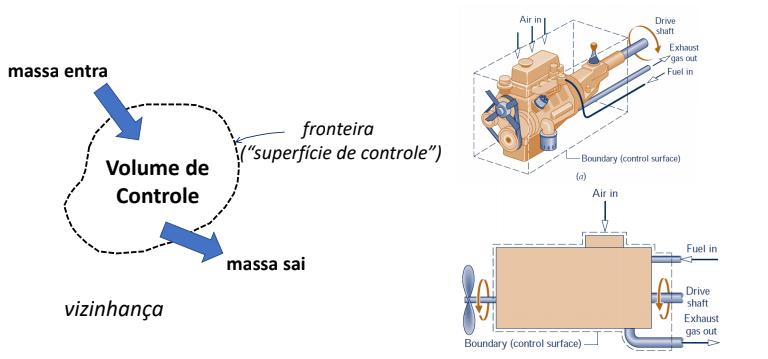
\includegraphics[width=10cm]{vc.png}
				\centering
				\caption{Volume de Controle}
			\end{figure}
	\end{enumerate}

\paragraph{Propriedades, Estado, Processo, Ciclo, Equilíbrio} 
	\begin{itemize}
		\item \textbf{Propriedade} é uma característica macroscópica de um sistema, à qual pode
		ser atribuído um valor numérico que independe da história prévia do
		sistema. Exemplos: massa, volume, pressão, temperatura, etc.
		
		\item \textbf{Estado} é a condição em que se encontra um sistema, descrita por suas
		propriedades.
		
		\item Quando uma ou mais propriedades variam, diz-se que o sistema passa por
		uma mudança de estado, ou \textbf{processo}.
		Notar que um sistema pode interagir continuamente com sua vizinhança
		sem contudo variar em suas propriedades. Neste caso, diz-se que o sistema
		está operando em \textbf{regime permanente}.
		
		\item \textbf{Equilíbrio} é a condição física interna em que um sistema, \textbf{isolado de sua
		vizinhança}, não apresenta alteração em suas propriedades. O equilíbrio é
		indicador de uniformidade interna nas propriedades do sistema
		(exemplo: temperatura, pressão), caso contrário ocorreriam movimentos
		internos, até a completa uniformização.
		
		Processos \textit{quasestáticos} podem ser considerados como sucessões de estados de equilíbrio.
	\end{itemize}

\paragraph{Propriedades Extensivas e Intensivas}
	\begin{itemize}
		\item Uma propriedade é \textbf{extensiva} quando o seu valor para
		o sistema é a soma dos valores dessa propriedade nas
		partes que compõem o sistema. Exemplos: a massa de
		um sistema é a soma das massas das partes
		constituintes do sistema.
		
		\item Uma propriedade \textbf{intensiva} expressa, como o nome
		diz, uma intensidade e assim, mesmo que seu valor
		mude de uma porção a outra do sistema, não pode
		ser somada. Exemplos: pressão, temperatura,
		qualquer propriedade extensiva dividida pela massa.
	\end{itemize}

\subsection{Propriedades PVT}
	\begin{enumerate}
		\item \textbf{Volume Específico:} $ v = \frac{1}{\varphi} = \frac{dV}{dm} $
		\item \textbf{Pressão:} $ p = \frac{dF}{dA} $
			\begin{itemize}
				\item Pressão Absoluta: A pressão que deve ser usada em todos os cálculos termodinâmicos é sempre a pressão absoluta p.
			\end{itemize}
			\begin{figure}[h]
				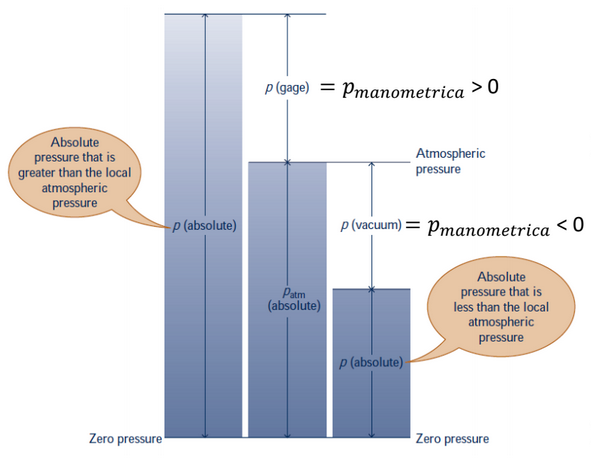
\includegraphics[width=10cm]{pa.png}
				\centering
				\caption{Pressão Absoluta x Pressão Manométrica}
			\end{figure}
		\item \textbf{Temperatura:} Quantidade associada à nossa sensação de calor e frio. Quando dois corpos estão em equilíbrio térmico
		com um terceiro, eles estarão em equilíbrio térmico entre si. \textbf{(“Lei Zero”)}
	\end{enumerate}

\newpage
\section{Capítulo 2 - Energia e Primeira Lei da Termodinâmica}

\subsection{Trabalho e Energia em Sistemas Mecânicos}
	\begin{enumerate}
		\item \textbf{Trabalho} é todo intercâmbio entre o sistema e a vizinhança  que pode ser descrito na forma:
		\begin{center}
			\large
			$ W = \int F*dr $
		\end{center}
		onde \textit{F} é a força e \textit{dr} o deslocamento associado a essa força.
		
		\item \textbf{Energia Potencial} se a força for tomada como o peso do corpo rígido:
		\begin{center}
			\large
			$ W_{gravidade} = mg(z_{1}-z_{2}) $
		\end{center}
	
		\item \textbf{Convenção de Sinais}
			\begin{figure}[h]
				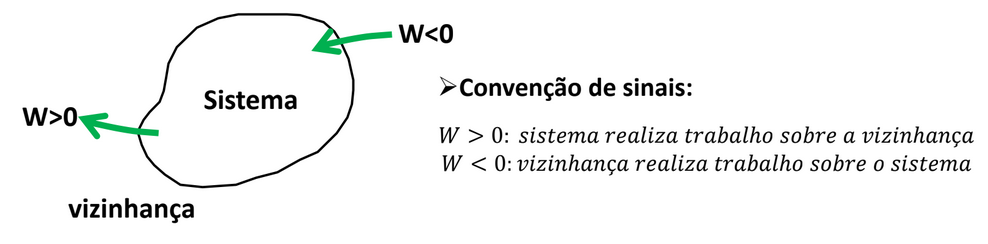
\includegraphics[width=15cm]{cs.png}
				\centering
				\caption{Conveção de Sinais}
			\end{figure}
			
		\item \textbf{Trabalho de Compresão/Expansão}\\
			\begin{center}
				\large
				$ W = \int p*dV $
			\end{center}

			\begin{figure}[h]
				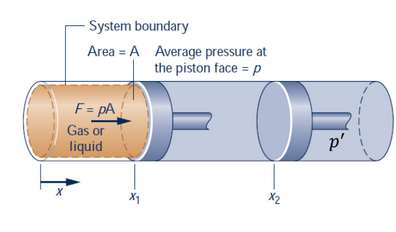
\includegraphics[width = 10cm]{tc.png}
				\centering
				\caption{Trabalho realizado pela pressão}
			\end{figure}
		
		\newpage
		\item \textbf{Trabalho em Processos Quase-Estáticos Politrópicos} O uso de uma relação do tipo $ p*V^{n} = const $ denominada \textit{processo politrópico}, permite calcular \textit{W} analiticamente.
			\begin{figure}[h]
				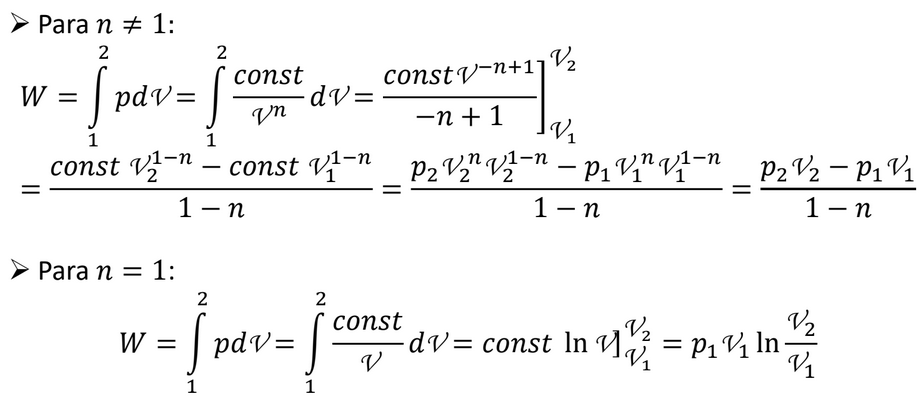
\includegraphics[width = 10cm]{pp.png}
				\centering
				\caption{Maneiras de Calcular o trabalho para Processos Politrópicos}
			\end{figure}
		 
	\end{enumerate}

\subsection{Energia Interna, Calor e Conservação de Energia em Sistemas Fechados}
\textbf{Energia Interna} é a energia acumulada no interior de um sistema fechado e que não pode ser expressa como energia cinética ou potencial gravitacional de seu CM.

	\begin{center}
		\large
		$ U =  $\textit{ energia interna}\\
		$ u =  $\textit{ energia interna específica}
	\end{center}

\textbf{Energia Total} de um sistema fechado é constituída pela soma das energias interna,
cinética e potencial gravitacional.
	\begin{center}
		\large
		$ E = U + \frac{mV^{2}}{2} + mgz$ \textit{energia total(extensiva)}\\
		$ e = u + \frac{V^{2}}{2} + gz$ \textit{energia total específica(intensiva)}
	\end{center}

\textbf{Calor} é toda forma de intercâmbio energético entre um sistema e sua
vizinhança que pode ser atribuído unicamente à diferença de temperatura entre ambos.
	\begin{figure}[h]
		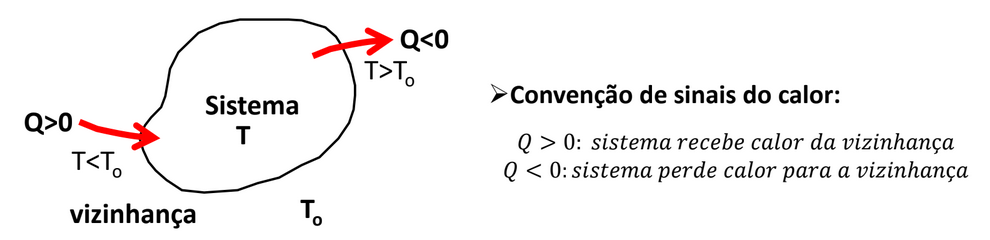
\includegraphics[width = 15cm]{ca.png}
		\centering
		\caption{Convenção de Sinais}
	\end{figure}

\textbf{Balanço de Energia em Sistemas Fechados}
	\begin{center}
		\large 
		$ E_{2} - E_{1} = Q - W $\\ ou\\
		$ m(e_{2} - e_{1}) = Q - W$
	\end{center}

\subsection{Aplicações da 1ª Lei da Termodinâmica}
\textbf{Sistemas Operando em Ciclos:}
Em um ciclo, por definição, o sistema retorna ao estado inicial após o ciclo ter
ocorrido. Logo:
	\begin{center}
		\large
		$ E_{2} = E_{1} \Rightarrow W_{ciclo} = Q_{ciclo}$
	\end{center}

\textbf{Ciclo de Potência:} A finalidade deste tipo de ciclo é gerar trabalho
mecânico a partir de uma fonte de calor qualquer,
conforme a figura. Usa água como fluido de trabalho.
	\begin{figure}[h]
		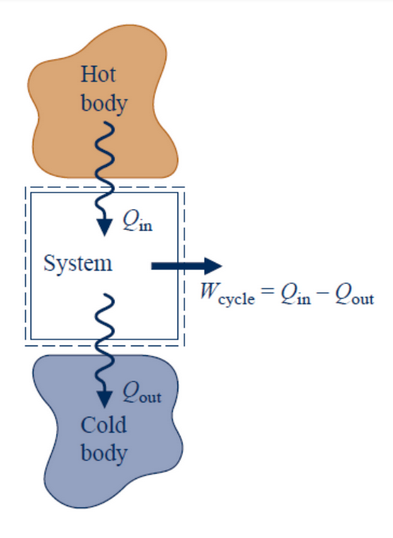
\includegraphics[width = 5cm]{cp.png}
		\centering
		\caption{Ciclo de Potência}
	\end{figure}

A primeira lei fica:
	\begin{center}
		\large
		$ W_{ciclo}  = Q_{in} - Q_{out}$
	\end{center}

A eficiência térmica do ciclo é definida por:
	\begin{center}
		\large
		$ n = \frac{W_{ciclo}}{Q_{in}} = 1 - \frac{Q_{out}}{Q_{in}} $
	\end{center}

\newpage
\textbf{Ciclo de Refrigeração e Bomba de Calor:} A finalidade deste tipo de ciclo é retirar calor de um corpo frio (refrigeração) e injetar calor em um corpo quente (bomba de calor), consumindo trabalho mecânico. Usa um “freon” como fluido de trabalho.
	\begin{figure}[h]
		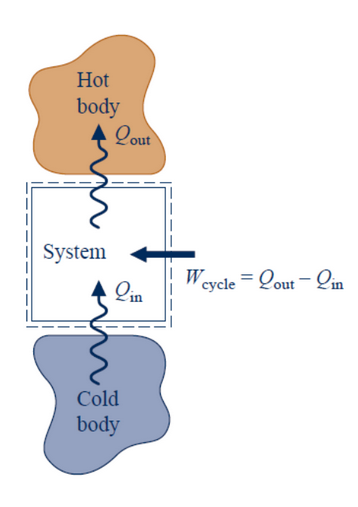
\includegraphics[width = 5cm]{cr.png}
		\centering
		\caption{Ciclo de Refrigeração}
	\end{figure}

A primeira lei fica:
	\begin{center}
		\large
		$ W_{ciclo}  = Q_{out} - Q_{in}$
	\end{center}

A eficiência térmica do ciclo é definida por:
	\begin{center}
		\large
		Refrigerador: $ \beta = \frac{Q_{in}}{W_{ciclo}} $ $ = \frac{Q_{in}}{Q_{out} - Q_{in}} $\\
		Bobma de Calor: $ \gamma  = \frac{Q_{out}}{W_{ciclo}} = \frac{Q_{out}}{Q_{out} - Q_{in}}$
	\end{center}


\newpage
\section{Capítulo 3 - Propriedades Termodinâmicas}
\subsection{Diagramas de Estado e Tabelas de Propriedades}
\textbf{Questões Importantes}
	\begin{enumerate}
		\item Dadas duas propriedades intensivas, em que fase a
		substância se encontra?
		
		\item Como obter suas outras propriedades?
		
		\item Por que bastam duas propriedades intensivas para
		definir o estado termodinâmico de uma substância?
	\end{enumerate}

	\begin{figure}[h]
		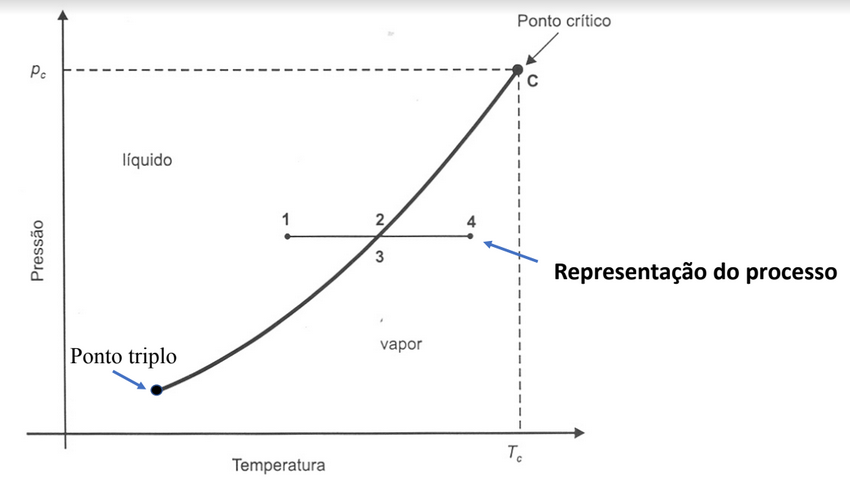
\includegraphics[width = 12cm]{pt.png}
		\centering
		\caption{Diagrama p-T de uma substância pura}
	\end{figure}

	\begin{figure}[h]
		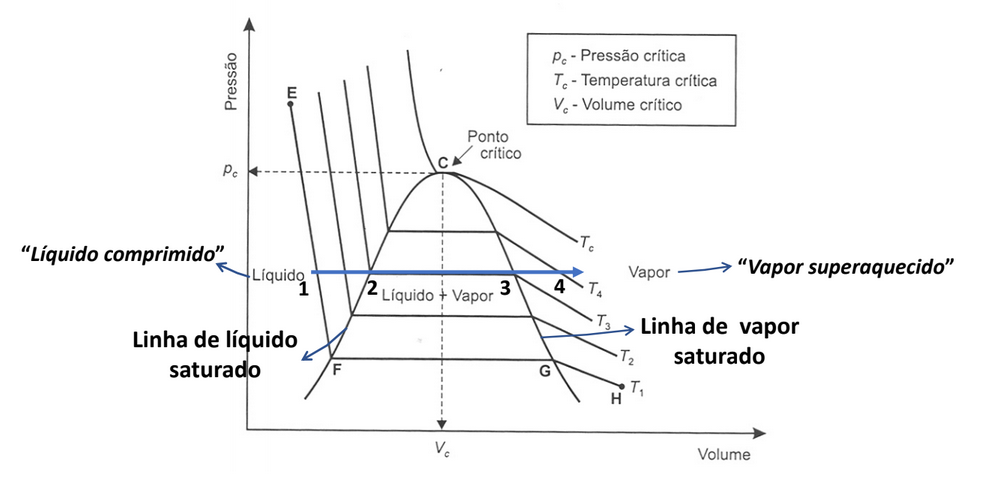
\includegraphics[width = 14cm]{pv.png}
		\centering
		\caption{Diagrama p-v de uma substância pura}
	\end{figure}

\textbf{Título de uma Mistura Líquido-Vapor}\\
Título é a fração em massa de vapor na mistura:

	\begin{center}
		\large
		$ x = \frac{massaVapor}{massaLiquido + massaVapor} = \frac{m_{g}}{m_{f} + m_{g}}$
	\end{center}	

\textbf{Volume específico de uma mistura L-V}\\
	\begin{center}
		\large
		$ v = xv_g+(1 - x)v_f $ \\
		Analogamente para a energia interna específica de uma mistura L-V
		$ u = xu_g+(1 - x)u_f $ \\ 
	\end{center}

\textbf{Cálculo Reverso do Título de uma Mistura}
	\begin{center}
		\large
		$ x = \frac{v - v_f}{v_g - v_f} $
	\end{center}

\textit{Obs:}
	\begin{itemize}
		\item Se o cálculo de x resultar $ > $ 1, é porque v $ > $ vg \textit{(vapor superaquecido)}
		
		\item Se x resultar $ < $ 0, é porque v $ < $ vf \textit{(líquido comprimido)}
	\end{itemize}

\textbf{Definição de Entalpia:} Processos a Pressão Constante\\
Pela 1ª Lei
	\begin{center}
		\large
		$ Q = U_2 + U_1 + p(V_2-V_1)  = (U_2+p_2V_2) - (U_1+p_1V_1) \Rightarrow$\\
		$ Q = H_2-H_1 = m(h_2-h_1) $
	\end{center}

\subsection{Modelos para Descrição de Propriedades}
\textbf{Calor Específico - Definição}\\
1ª Lei para um processo de troca de calor a volume constante: $ Q = m(u_2-u_1)$. Define-se \textit{calor específico a volume constante}:
	\begin{center}
		\large
		$ c_v = \frac{\delta u}{\delta T} $
	\end{center}

1ª Lei para um processo de troca de calor a pressão constante: $ Q = m(h_2-h_1) $. Define-se \textit{calor especifico a pressao constante}:
	\begin{center}
		\large
		$ c_p = \frac{\delta h}{\delta T} $
	\end{center}

\textbf{Modelo de Substância Incompressível}\\
É toda substância que não muda de fase e para a qual o volume específico não varia ao longo do processo.
A síntese das equações que descrevem este tipo de substância é:
	\begin{center}
		\large
		$ v = const $\\
		$ c_p = c_v = c $\\
		$ u_2 - u_1 = c_{medio}(T_2 - T_1) $\\
		$ h_2 - h_1 = c_{medio}(T_2-T_1) + v(p_2-p_1) $
	\end{center}

\textbf{Modelo de Gás Ideal}\\
A síntese das equações que descrevem este tipo de substância é:
	\begin{center}
		\large
		$ pv = RT $, onde $ R = \frac{8,314 \frac{kJ}{kmol k}}{M} $\\
		$ k = \frac{c_p}{c_v} \Rightarrow c_v = \frac{R}{k - 1} $; $c_p = \frac{kR}{k - 1} $\\
		$ u_2 - u_1 = c_{v,medio}(T_2-T_1) $\\
		$ h_2-h_1 = c_{p,medio}(T_2-T_1) $
	\end{center}


\newpage
\section{Capítulo 4 - Análise de Volume de Controle}
\subsection{Conservação de Massa em Volume de Controle}
\textbf{Situação Típica de um Escoamento}\\
Durante um escoamento, um sistema fechado (móvel) pode ser arbitrariamenteescolhido para análise. Uma vez escolhido, sua massa é sempre a mesma.

O processo que ocorre quando esse sistema fechado passa uma região arbitrária
do espaço (VC) é o que desejamos analisar.
	\begin{figure}[h]
		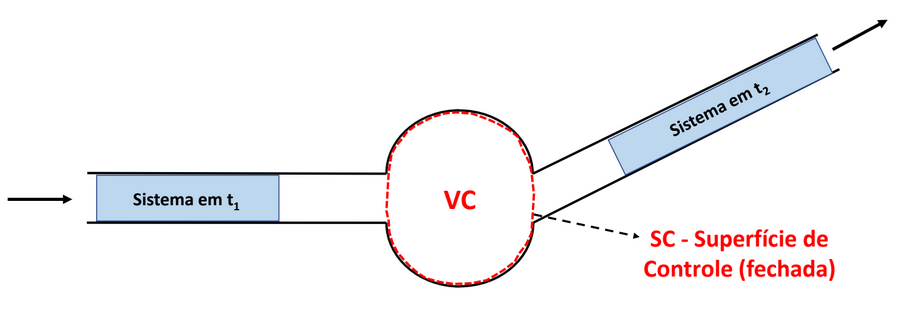
\includegraphics[width = 12cm]{vcc.png}
		\centering
		\caption{Escoamento}
	\end{figure}
	
Para um Volume de Controle com várias entradas e saídas:
	\begin{center}
		\large
		$ \frac{dm_{vc}}{dt} = \sum\limits_{entradas}\dot{m_{in}} - \sum\limits_{saidas}\dot{m_{out}}$
	\end{center}

\textbf{Dois tipos de Vazão:}\\
	\begin{center}
		\large
		\textbf{Vazão em Volume}\\
		$ \dot{V_{vol_{in}}} = A_{in}V_{in} $\\
		$ \dot{V_{vol_{out}}} = A_{out}V_{out} $\\
		
		\textbf{Vazão em Massa}\\
		$ \dot{m}_{in} = \frac{\dot{V_{vol_{in}}}}{v_{in}} = \varphi_{in}A_{in}V_{in} $\\
		$ \dot{m}_{out} = \frac{\dot{V_{vol_{out}}}}{v_{out}} = \varphi_{out}A_{out}V_{out} $
	\end{center}

\subsection{Conservação de Energia em Volume de Controle}
Para um VC com várias entradas e saídas:
	\begin{center}
		\large
		$ \frac{dE_{vc}}{dt} = \dot{Q} - \dot{W} + \sum\limits_{entradas}\dot{m}_i(h_i + \frac{V_i^2}{2} + gz_i) - \sum\limits_{entradas}\dot{m}_o(h_o + \frac{V_o^2}{2} + gz_o) $
	\end{center}
A equação acima representa a 1a Lei da Termodinâmica para um VC genérico.

Notar que a única diferença em relação à 1a Lei para \textbf{sistema fechado} é a
presença dos \textbf{termos de entrada e saída} de fluido através da superfície de
controle.\\

Para o caso de \textbf{regime transiente}, onde as propriedades internas do sistema permanecem constantes:
	\begin{center}
		\large
		$ \frac{dm_{vc}}{dt} = \frac{dE_{vc}}{dt}$
	\end{center}

\subsection{Aplicações das Leis de Conservação da Massa e da Energia em Regime Permanente}
	\begin{enumerate}
		\item Turbinas a Vapor/Turbinas a Gás;
		\item Compressores;
		\item Trocadores de Calor;
		\item Válvulas e dispositivos de estrangulamento;
		\item Bocais e difusores;
		\item Integração de Dispositovos:
			\begin{itemize}
				\item Ciclo de Potência a Vapor;
				\item Ciclo de Refrigeração.
			\end{itemize}
	\end{enumerate}


\subsection{Aplicações da Conservação da Massa e Energia em Regime Transiente}
	\begin{center}
		\large
		$ m_{VC,t} - m_{VC,0} = \sum\limits_{entradas}m_i - \sum\limits_{saida}m_o$
	\end{center}

\textbf{Caso A: Entalpia de Entrada/Saída Constante com o Tempo}\\
	\begin{center}
		\large
		$ m_{VC,t}u_{VC,t} - m_{VC,0}u_{VC,0} = Q - W + \sum\limits_{entradas}m_ih_i - \sum\limits_{saida}m_oh_o $
	\end{center}

\textbf{Caso B: Propriedades Intensivas Uniformes no VC}\\
	\begin{center}
		\large
		$ \int_{0}^{t} m_{VC}\frac{dh_{VC}}{dt}dt - (pV)_{VC,t} + (pV)_{VC,0} = Q - W$
	\end{center}


\newpage
\section{Capítulo 5 - Segunda Lei da Termodinâmica}
\subsection{Segunda Lei da Termodinâmica}
\textbf{Carnot}\\
“No machine or combination of machines
can ever have the effect of making more
heat run up to high temperature than
down to low temperature.”\\

Analogia com duas rodas d’água
operando juntas.

	\begin{figure}[h]
		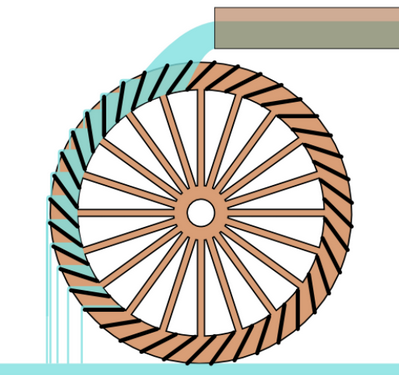
\includegraphics[width = 8cm]{cc.png}
		\centering
		\caption{Analogia com Rodas d'água}
	\end{figure}

\textbf{Clausius}\\
“É impossível para qualquer
sistema operar de tal forma que o
\textbf{único} resultado seja a transferência
de calor de um corpo frio para um
corpo quente.”

	\begin{figure}[h]
		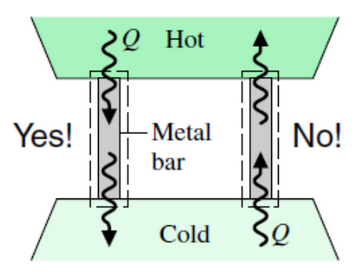
\includegraphics[width = 8cm]{caca.png}
		\centering
		\caption{Processo Impossível}
	\end{figure}

\newpage
\textbf{Kelvin-Planck}\\
“É impossível para qualquer sistema
operar em um ciclo termodinâmico e
entregar um trabalho líquido à sua
vizinhança enquanto recebe calor de
um único reservatório térmico.”

	\begin{figure}[h]
		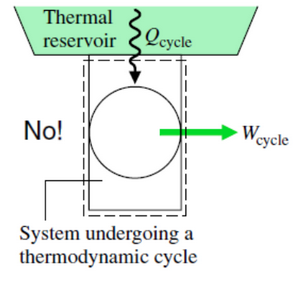
\includegraphics[width = 6cm]{kp.png}
		\centering
		\caption{Processo Impossível}
	\end{figure}

\subsection{A Melhor Máquina Térmica}
\textbf{Processo Irreversível}\\
É aquele em que o sistema e a sua vizinhança não podem retornar a seus estados
iniciais após o processo ter ocorrido.

É possível que ou o sistema ou a vizinhança retornem ao estado em que
se encontravam inicialmente, mas não ambos

Todos os processos que ocorrem \textbf{espontaneamente} são irreversíveis, pois
revertê-los irá requer trabalho da vizinhança sobre o sistema.\\

Todos os processos reais são irreversíveis, em maior ou menor grau.\\

A escolha da fronteira do sistema é fundamental para definir o tipo e a
localização das irreversibilidades. Quando um fluido de trabalho está
envolvido, este é geralmente escolhido como o sistema.\\

\textbf{Processos Reversíveis}\\
São aqueles em que o sistema e a sua vizinhança podem ser
exatamente restaurados a seus estados iniciais após o processo ter
ocorrido.
São processos puramente hipotéticos, como um caso-limite.\\

\textbf{Processos Internamente Reversíveis}\\
São aqueles em que a fronteira é escolhida de tal forma que não há irreversibilidades
no interior do sistema.

Além disso, cada estado percorrido é tal que todas as suas propriedades intensivas são
uniformes ao longo do sistema.

Devem, portanto, ser processos lentos, quasiestáticos.\\

\textbf{Aplicação da 2ª Lei a Ciclos(máquinas térmicas)}\\

\textbf{Ciclos com um Resevatório}\\
Enunciado de Kelvin-Planck:\\
“É impossível para qualquer sistema operar em
um ciclo termodinâmico e entregar um
trabalho líquido à sua vizinhança enquanto
recebe calor de um único reservatório térmico.”
	\begin{center}
		\large
		$ W_{ciclo} \leq 0$
	\end{center}

	\begin{figure}[h]
		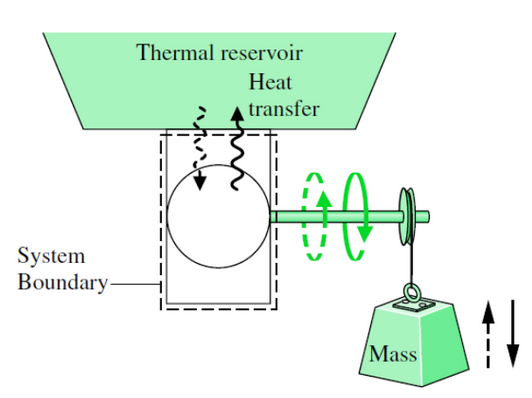
\includegraphics[width = 10cm]{re.png}
		\centering
		\caption{O ciclo indicado pelas linhas pontilhadas
			não pode ocorrer.}
	\end{figure}

\textbf{Ciclos de Potência com 2 Reservatórios}\\

Pelo enunciado de Kelvin-Planck, $ Q_c $ não pode ser nulo!\\

Eficiência térmica do ciclo
(usando valores em módulo!):
	\begin{center}
		\large
		$ n = \frac{W_{ciclo}}{Q_H} = \frac{Q_H - Q_C}{Q_H} $\\
		$ n = 1 - \frac{Q_C}{Q_H} $
	\end{center}

\textbf{Corolários de Carnot para Ciclos de Potência}
	\begin{enumerate}
		\item A eficiência térmica de um ciclo de potência irreversível é sempre inferior
		à de um ciclo de potência reversível entre os mesmos dois reservatórios;
		\item Todos os ciclos de potência reversíveis operando entre os mesmos dois
		reservatórios térmicos têm a mesma eficiência térmica.
	\end{enumerate}
	
	\begin{figure}[h]
		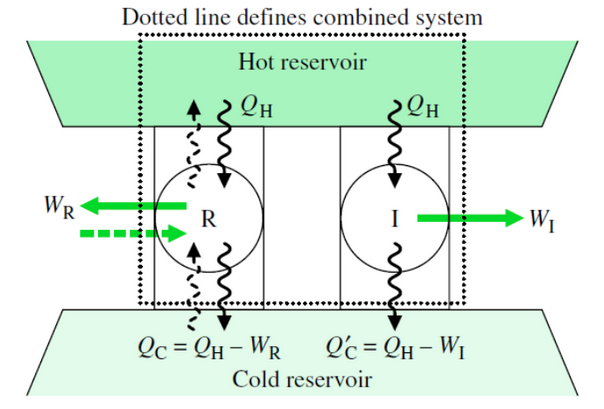
\includegraphics[width = 10cm]{rr.png}
		\centering
		\caption{O sistema combinado indicado troca
			calor apenas com o reservatório frio}
	\end{figure}
	
\newpage
\textbf{Ciclos de Refrigeração com 2 Reservatórios}\\
Pelo enunciado de Clausius, $ W_{ciclo} $ não pode ser nulo!\\

Se o objetivo é refrigerar, o coeficiente
de performance é definido por:
	\begin{center}
		\large
		$ \beta = \frac{Q_C}{W_{ciclo}} =  \frac{Q_C}{Q_H - Q_C} = \frac{1}{\frac{Q_H}{Q_C} - 1}$
	\end{center}
Se o objetivo é bombear calor, o coeficiente
de performance é definido por:
	\begin{center}
		\large
		$ \gamma = \frac{Q_H}{W_{ciclo}} = \frac{Q_H}{Q_H - Q_C} = \frac{1}{1 - \frac{Q_C}{Q_H}}$
	\end{center}
	
\textbf{Corolários de Carnot para Ciclos de Refrigeração/Bombeio de Calor}
	\begin{enumerate}
		\item O coeficiente de performance de um ciclo de refrigeração irreversível é
		sempre inferior ao de um ciclo de refrigeração reversível entre os mesmos
		dois reservatórios;
		\item Todos os ciclos de refrigeração reversíveis operando entre os mesmos
		dois reservatórios térmicos têm o mesmo coeficiente de performance.
	\end{enumerate}
	
	\begin{figure}[h]
		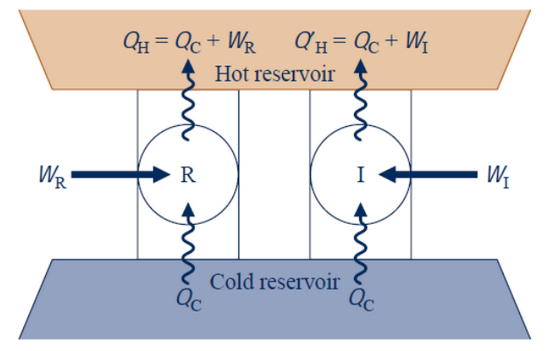
\includegraphics[width = 10cm]{rb.png}
		\centering
		\caption{Neste caso, o conjunto 
			operaria trocando calor apenas com o
			reservatório quente}
	\end{figure}
	
\newpage
\subsection{Ciclo de Carnot}
\textbf{Melhor Desempenho de um Ciclo Operando entre Dois Reservatórios Térmicos}
	\begin{center}
		\large
		Ciclo de Potência: $ n_{max} = 1 - \frac{T_C}{T_H} $\\
		Ciclo de Refrigeração: $ \beta_{max} =  \frac{1}{\frac{T_H}{T_C} - 1} $\\
		Ciclo de Calor: $ \frac{1}{1 - \frac{T_C}{T_H}} $
	\end{center}
	
\textbf{Desigualdade de Clausius}
	\begin{center}
		\large
		$ \int_{ciclo} (\frac{\delta Q}{T})_b \leq 0$,\\ onde "b"  representa “calculado na fronteira do
		sistema.”
	\end{center}
	
\textbf{Quantificação da Irreversibilidade de um Ciclo}\\
Pode-se escrever a desigualdade de Clausius como uma igualdade:
	\begin{center}
		\large
		$ \int_{ciclo} (\frac{\delta Q}{T})_b = -\sigma_{ciclo}$\\
		Ou em termos de taxa:\\
		$ \int_{ciclo} (\frac{\delta \dot{Q}}{T})_b = -\dot{\sigma}_{ciclo}$
	\end{center}
	Onde:\\
	$ \sigma_{ciclo} = 0 $: sem irreversibilidades internas (ciclo internamente reversivel);\\
	$ \sigma_{ciclo} > 0 $: irreversibilidades presentes dentro do sistema;	\\
	$ \sigma_{ciclo} < 0 $: ciclo impossivel.\\
	
	$ \sigma_{ciclo} $ representa a intensidade das irreversibilidades presentes no interior do sistema,	ou seja, quanto maior for $ \sigma_{ciclo} $, mais ineficiente é o ciclo.
	

\newpage
\section{Capítulo 6 - Entropia}
\subsection{Entropia: Definição Macroscópica}
\textbf{Variação de Entropia}
	\begin{center}
		\large
		$ S_2 - S_1 = \int_{1}^2 (\frac{\delta Q}{T})_{int. reversivel} $  $ [\frac{J}{K}] $ 
	\end{center}

\textbf{Calor e Trabalho em Processos Internamente
	Reversíveis de um Sistema}\\

Por definição:
	\begin{center}
		\large
		$ dS = (\frac{\delta Q}{T})_{int. reversivel} \Rightarrow
		Q_{int.reversivel} = \int^2_{1}TdS $
	\end{center}
Assim, se o processo for \textbf{adiabático reversível}, ele será \textit{isentrópico}.

Da mesma forma, para um sistema constituído por uma substância
compressível simples:
	\begin{center}
		\large
		$ \delta W = pdV \Rightarrow 
		W_{int.reversivel} = \int^2_1 pdV $
	\end{center}

\subsection{Modelos para Cálculo de Entropia}
\textbf{Equações Tds}
	\begin{center}
		\large
		$ Tds = du + pdv $ ou
		$ Tds = dh  - vdp $
	\end{center}

\textit{s} tende a aumentar quando: aumento em T, aumento em v, redução em p
(quanto maior a “mobilidade” do fluido, maior a entropia)

\textbf{Variação de Entropia para um Gás Ideal}
	\begin{center}
		\large
		$ ds = \frac{c_vdT}{T} + \frac{R}{v}dv $\\
		$ ds = \frac{c_pdT}{T} - \frac{R}{p}dp$
	\end{center}

\textbf{Uso das Tabelas de Gás Ideal}
	\begin{center}
		\large
		$ s_2 - s_1 = s^\circ(T_2) - s^\circ(T_1) - Rln\frac{p_2}{p_1}$
	\end{center}

\textbf{Gás Ideal com Calores Específicos Constantes}
	\begin{center}
		\large
		$ s_2 - s_1 = c_vln\frac{T_2}{T_1} + Rln\frac{v_2}{v_1} $\\
		$ s_2 - s_1 = c_pln\frac{T_2}{T_1} - Rln\frac{p_2}{p_1} $
	\end{center}

Lembrar que, para gases ideais:
	\begin{center}
		\large
		$ c_p - c_v = R $ ;$ c_p = \frac{kR}{k - 1} $ ;$ c_v = \frac{R}{k - 1} $
	\end{center}

\textbf{Variação de Entropia de uma Substância Incompressível (ex: sólidos e líquidos sem mudança de fase)}
	\begin{center}
		\large
		$ s_2 - s_1 = cln\frac{T_2}{T_1} $
	\end{center}

\subsection{Balanço de Entropia para Sistema Fechado}
\textbf{2ª Lei para Sistema Fechado: Balanço de Entropia}
	\begin{center}
		\large
		$ S_2 - S_1 = \int^2_1(\frac{\delta Q}{T})_b + \sigma_{12} $
	\end{center}

Onde,
	\begin{flushleft}
		$ \sigma_{12} = 0$: processo internamente reversível\\
		$ \sigma_{12} > 0$: irreversibilidades internas\\
		$ \sigma_{12} < 0$: processo impossível
	\end{flushleft}
	
Pela figura abaixo:

	\begin{figure}[h]
		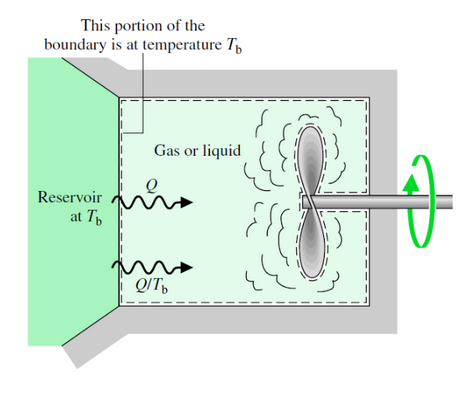
\includegraphics[width = 8cm]{aa.png}
		\centering
		\caption{Exemplo de um reservatório}
	\end{figure}	

	\begin{center}
		\large
		$ S_2 - S_1 = \int^2_1(\frac{\delta Q}{T})_b + \sigma_{12} = \frac{Q}{T_b} + \sigma $
	\end{center}

$ \sigma  $ é a \textbf{geração de entropia} do processo(medida da irreversibilidade interna) e \textit{nunca} é negativa.

\textbf{Sistema Isolado}
Um sistema é dito isolado quando não interage via calor ou trabalho com sua vizinhança. Pela 1ªLei:
	\begin{center}
		\large
		$ E_2 - E_1 = Q_{(=0)} - W_{(=0)} \Rightarrow E_2 = E_ 1$
	\end{center}
E pela 2ªLei:
	\begin{center}
		\large
		$ S_2 - S_1 = \int^2_1(\frac{\delta Q}{T})_b + \sigma_{12} \Rightarrow S_2\geq S_1$
	\end{center}

\begin{itemize}
	\item Um sistema isolado deve evoluir para um estado de equilíbrio caracterizado pela uniformidade em suas propriedades;
	\item Assim, as irreversibilidades se tornam cada vez menores à medida que o sistema se aproxima do equilíbrio. Ou seja, $ \sigma $ diminui conforme o equilíbrio é aproximado;
	\item Dessa forma, no estado de equilíbrio, a entropia de um sistema isolado deve ser máxima. Este é o princípio do aumento da entropia para um sistema isolado.
\end{itemize}

\textbf{Formas do Balanço de Entropia para Sistemas Fechados}
	\begin{center}
		\large
		$ S_2 - S_1 = \sum_{j}^{} \frac{Q_j}{T_j} + \sigma$\\
		
		$ dS = \sum_{j}^{} \frac{\delta Q_j}{T_j} + \delta \sigma $\\
		
		$ \frac{dS}{dt} = \sum_{j}^{} \frac{\dot{Q_j}}{T_j} + \dot{\sigma} $
	\end{center}

\subsection{Balanço de Entropia para Volume de Controle}
\textbf{Balanço de Entropia para VC}
Para volumes de controle, é necessário acrescentar as entropias que entram e saem junto com as respectivas vazões em massa nas entradas e saídas. Assim, para VC:
	\begin{center}
		\large
		$ \frac{dS_{VC}}{dt} = \sum_{j} \frac{\dot{Q}_j}{T_j} + \sum_{entradas} \dot{m}_is_i - \sum_{saidas} \dot{m}_os_o + \dot{\sigma} $
	\end{center}

\subsection{Escoamento Isentrópico}
\textbf{Escoamento Isentrópico – Conceito}\\
É todo escoamento que ocorre de forma \textbf{adiabática} e \textbf{internamente reversível}. Portanto, teremos:
	\begin{center}
		\large
		$ s_2 = s_1 $
	\end{center}

Este tipo de escoamento é utilizado como “\textit{ideal a atingir}” para turbinas,
compressores, bombas, bocais e outros dispositivos termicamente isolados.

Além disso, qualquer escoamento em regime transiente, que ocorra de forma
\textit{adiabática} e seja \textit{suficientemente lento} para que as propriedades no interior
do VC sejam uniformes, pode ser considerado isentrópico no interior do VC.
Isto se justifica pois, neste caso, $ s_i = s_o = s_{VC} $.

\textbf{Escoamento Isentrópico de Gases Ideais com Calores Específicos Variáveis}\\
	\begin{center}
		\large
		$ s^{\circ}(T_2) = s^{\circ}(T_1) + Rln\frac{p_2}{p_1} $ ou $ \frac{p_2}{p_1} = e^{\frac{s^{\circ}(T_2) - s^{\circ}(T_1)}{R}} $
	\end{center}
Para ar como gás ideal, a Tab. A-22 fornece valores da função $ s^{\circ} $(T), permitindo resolver a equação acima para T ou p.\\

\textbf{Escoamento Isentrópico de Gases Ideais com Calores Específicos Constantes}\\
Para obter o estado final basta utilizar as relações:
	\begin{center}
		\large
		$ \frac{T_2}{T_1} = (\frac{v_1}{v_2})^{k - 1} $\\
		$ \frac{T_2}{T_1} = (\frac{p_2}{p_1})^{\frac{k-1}{k}} $
	\end{center}

Ou, dividindo uma relação pela outra:
	\begin{center}
		\large
		$ \frac{p_2}{p_1} = (\frac{v_1}{v_2})^k $ isto é $ pv^k = const $
	\end{center}

	\begin{figure}[h]
		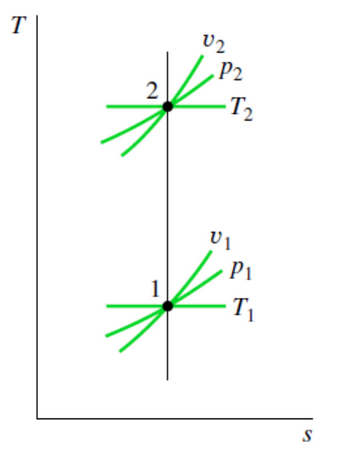
\includegraphics[width = 6cm]{BB.png}
		\centering
		\caption{Estados inicial e final}
	\end{figure}

\newpage
\textbf{Escoamento Politrópico de um Gás}
Podemos generalizar a relação do escoamento isentrópico:
	\begin{center}
		\large
		$ pv^k = const $
	\end{center}
para uma única expressão capaz de descrever diversos tipos de escoamentos
\textit{internamente reversíveis} de um gás:
	\begin{center}
		\large
		$ pv^n = const $
	\end{center}

Dessa forma, para um gás ideal ($ pv = RT $) o valor de \textit{n} se ajusta a diversas
situações:
	\begin{center}
		$ n = 0: $ escoamento isobárico $ \leftrightarrow p = const $\\
		$ n = 1: $ escoamento isotérmico $ \leftrightarrow T = const $\\
		$ n = k: $ escoamento isentrópico $ \leftrightarrow s = const $\\
		$ n = \pm \infty: $ escoamento incompressível $ \leftrightarrow v = const $\\
	\end{center}

	\begin{figure}[h]
		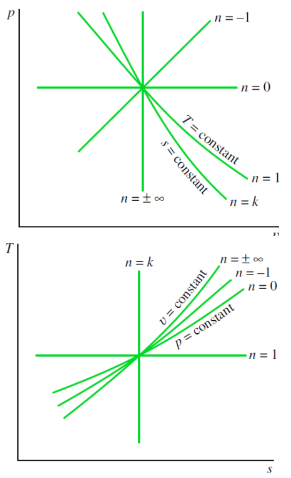
\includegraphics[width = 8cm]{ccc.png}
		\centering
		\caption{O uso de pv
			n = const com n ajustado a dados experimentais de um
			escoamento real, permite descrever esse escoamento ou dispositivo/máquina
			por meio de uma equação algébrica útil para representar seu comportamento
			termodinâmico.}
	\end{figure}

\newpage
\textbf{Calor e Trabalho em Escoamento Politrópico}
Considere um VC com uma entrada (“1”) e uma saída (“2”) operando em regime
permanente. Na hipótese de o VC operar sem irreversibilidades internas, o calor pode ser calculado por:
	\begin{center}
		\large
		$ \dot{Q}_{int.rev.VC} = \dot{m} \int_1^2 Tds$
	\end{center}

Para obtermos a potência mecânica, usamos o balanço de energia no VC.
	\begin{center}
		\large
		$ \dot{W}_{int.rev.VC} = -\dot{m}\int_{1}^{2}vdp $
	\end{center}

Integral essa que pode ser resolvida usando a relação $ pv^n = const $.\\Integrando:
	\begin{center}
		\large
		$ \frac{\dot{W}_{int.rev.VC}}{\dot{m}} = $
		$\left\{
		\begin{array}{cl}
			-\frac{n}{n - 1}(p_2v_2-p_1v_1) & n\neq 1\\
			-p_1v_1ln(\frac{p_2}{p_1}) & n = 1
		\end{array}
		\right.$
	\end{center}

Casos particulares:
	\begin{center}
		$ n = 0: $ escoamento isobárico $ \leftrightarrow  \dot{W}_{inv.rev.VC} = 0 $ 
		
		$ n = 1: $ escoamento isotérmico $ \leftrightarrow  \dot{W}_{inv.rev.VC} = -\dot{m}p_1v_1ln(\frac{p_2}{p_1}) $ 
		
		$ n = k: $ escoamento isentrópico $ \leftrightarrow  \dot{W}_{inv.rev.VC} = -\frac{\dot{m}k}{k-1}(p_2v_2-p_1v_1) $ 
		
		$ n = \pm\infty: $ escoamento incompressível $ \leftrightarrow  \dot{W}_{inv.rev.VC} = -\dot{m}v(p_2-p_1) $ 
	\end{center}

\subsection{Eficiência Isentrópica}
\textbf{Eficiência de um Dispositivo de Conversão de Energia}\\
É definida como a razão entre a energia convertida no dispositivo real e a convertida em um dispositivo ideal, obtendo sempre um número inferior a 1.

Assim, uma turbina nunca poderia gerar mais potência que a turbina ideal nas
mesmas condições.

Um compressor nunca poderia consumir menos potência que o compressor ideal nas
mesmas condições.

A razão disso são as irreversibilidades, internas e externas, presentes nas máquinas
reais.\\

\textbf{Eficiência Isentrópica de Turbinas Térmicas}
Qualquer perda de calor da turbina para a vizinhança, além de
irreversível, levaria a uma perda de eficiência na conversão de
entalpia em trabalho.
	\begin{center}
		\large
		$ n_t = \frac{\dot{W}/\dot{m}}{(\dot{W}/\dot{m})_s} = \frac{h_1 - h_2}{h_1 - h_{2s}}$ $ (\sim0.7 - 0.9) $
	\end{center}
As irreversibilidades internas fazem com que o fluido saia mais
quente ($ h_2 > h_{2s} $).
	\begin{figure}[h]
		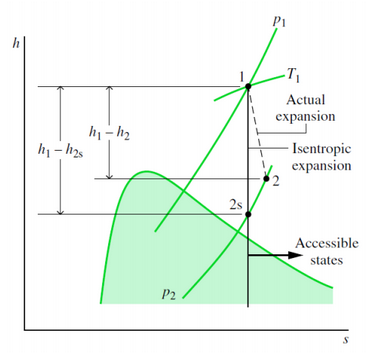
\includegraphics[width = 8cm]{hs.png}
		\centering
		\caption{Diagrama h-s}
	\end{figure}

\textbf{Eficiência Isentrópica de Bocais}\\
Bocais são dispositivos usados para converter energia de pressão em
energia cinética. São comumente usados em propulsão (aviões,
foguetes, etc). Essa conversão deve, idealmente, ocorrer sem perda de
calor para a vizinhança.
	\begin{center}
		\large
		$ n_{bocal} = \frac{V_2^2/2}{V^2_{2s}/2} $ 
		$ (>\sim 0.95) $
	\end{center}
	\begin{figure}[h]
		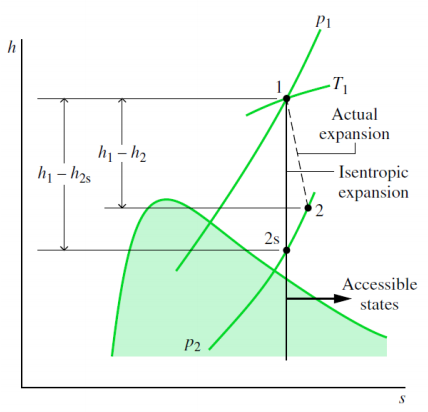
\includegraphics[width = 8cm]{hss.png}
		\centering
		\caption{Diagrama h-s}
	\end{figure}

\textbf{Eficiência Isentrópica de Compressores e Bombas}\\
Estas máquinas convertem energia mecânica em energia de
pressão. Essa conversão deve ocorrer sem perda de calor para
a vizinhança.
	\begin{center}
		\large
		$ n_c = \frac{(\dot{W}/\dot{m})_s}{\dot{W/\dot{m}}} = \frac{h_{2s} - h_1}{h_2 - h_1}$ $ (\sim0.75 - 0.85) $
	\end{center}

\newpage
\section{Interpolação Linear}
	\begin{center}
		\large
		$ y = y_0 + (y_1 - y_0)\frac{x - x_0}{x_1 - x_0} $
	\end{center}



\end{document}